%! TEX TS-program = lualatex
\documentclass[12pt,openright,oneside,a4paper,
	chapter=TITLE,
	section=TITLE,
	english,brazil]{abntex2}
\usepackage[alf]{abntex2cite}
\usepackage[T1]{fontenc}
\usepackage{fontspec}
\usepackage{graphicx}
\usepackage[none]{hyphenat}
\usepackage{hyperref}
\usepackage{indentfirst}

\setmainfont{Arial}
\setlength{\parindent}{1.5cm}
\setlength{\emergencystretch}{2cm}
\setlength{\cftbeforeparagraphskip}{0pt}
\setlength{\cftbeforesubsubsubsectionskip}{0pt}
\setlength{\cftbeforechapterskip}{0pt}
\setlength{\cftbeforesubsubsectionskip}{0pt}

\author{Heber Ferreira Barra \\ João Gabriel de Cristo}
\titulo{Trabalho de Pesquisa UML}
\date{2024}
\instituicao{Instituto Federal do Paraná}
\local{Curitiba}
\preambulo{Trabalho de pesquisa sobre diagramas UML.}
\tipotrabalho{pesquisa}
\orientador{MSc. Elaini Simoni Angelotti}

\makeatletter
\hypersetup{
    pdfauthor={\@author},
    pdfsubject={\imprimirpreambulo},
    pdfcreator={LaTeX with abntex2},
    colorlinks=true,
    linkcolor=black,
    urlcolor=blue,
	citecolor=black
}
\makeatother

\renewcommand{\ABNTEXchapterfont}{\bfseries\MakeUppercase\sffamily}
\renewcommand{\ABNTEXchapterfontsize}{\normal}
\renewcommand{\ABNTEXsectionfont}{\MakeUppercase\sffamily}
\renewcommand{\ABNTEXsectionfontsize}{\normal}
\renewcommand{\labelenumi}{\theenumi}
\renewcommand{\theenumi}{\Roman{enumi} -}%
\renewcommand{\authorcapstyle}{\normal}
\renewcommand{\cftsectionfont}{\normalfont\MakeUppercase}
\newcommand{\bibtextitlecommand}[2]{\bf{#2}}
\newcommand{\authorstyle}{\relax}

\renewcommand{\imprimircapa}{%
	\begin{capa}
		\center
		\ABNTEXchapterfont\bfseries\MakeUppercase\imprimirinstituicao\\
		\vspace*{1cm}
		\ABNTEXchapterfont\bfseries\MakeUppercase\imprimirautor
		\vfill
		\begin{center}
			\ABNTEXchapterfont\bfseries\MakeUppercase\imprimirtitulo
		\end{center}
		\vfill

		\bfseries\MakeUppercase\imprimirlocal

		\bfseries\MakeUppercase\imprimirdata

		\vspace*{1cm}
	\end{capa}
}

\makeatletter
\renewcommand{\folhaderostocontent} {
	\center
	{\normal\imprimirautor}

	\vspace*{\fill}
	\begin{center}
		\ABNTEXchapterfont\bfseries\MakeUppercase\imprimirtitulo
	\end{center}

	\abntex@ifnotempty{\imprimirpreambulo}{%
		\hspace{.45\textwidth}
		\begin{minipage}{.5\textwidth}
			\SingleSpacing
			\small\imprimirpreambulo \\
			\\
			\imprimirorientadorRotulo\ \imprimirorientador
		\end{minipage}
	}

	\vspace*{\fill}
	{\imprimirlocal}
	\par
	\imprimirdata
	\vspace*{1cm}
}
\makeatother

\begin{document}
\selectlanguage{brazil}
\imprimircapa
\imprimirfolhaderosto

\pdfbookmark[0]{\listfigurename}{lof}
\listoffigures*
\cleardoublepage

\pdfbookmark[0]{\contentsname}{toc}
\tableofcontents*
\cleardoublepage

\textual
\chapter{Introdução à UML}
De acordo com GUEDES(2018, pg. 22), a UML(Unified Modeling Language) é uma linguagem de modelagem visual, cujo objetivo é a modelação de softwares orientados a objetos, que pode ser aplicada a quaisquer tipos de aplicação. A UML visa auxiliar os engenheiros de software a definirem os aspectos de um sistema, desde os requisitos técnicos até os comportamentos do programa.

Esta linguagem foi o resultado da união dos três métodos de modelagem orientados a objeto mais utilizados, sendo estes: o método de Booch, o método OMT(Object Modeling Technique), criado por Jacobson, e o método OOSE(Object-Oriented Software Engineering) proposto por Rumbaugh. Desta união, surge a primeira versão da UML em 1996. 

Depois do lançamento da versão inicial, muitas empresas passaram a contribuir com o desenvolvimento da UML. No ano seguinte, a OMG(Object Management Group) adotou a linguagem como uma linguagem-padrão de modelagem. Posteriormente, no ano de 2005, foi lançada a UML 2.0.

Assim como é necessário planejamento para construir-se um prédio, também faz-se necessário planejamento para desenvolver softwares, especialmente os mais complexos, que possuem mais requisitos e funcionalidades complicadas. Pelos sistemas de informações serem extremamente dinâmicos, crescendo em funcionalidades e requisitos, de acordo com as demandas dos clientes, é ainda mais essencial que um programa seja bem modelado e tenha uma documentação detalhada, que seja constantemente atualizada e revisada, visando facilitar  a manutenção e expansão do sistema, sendo modelagem uma das melhores formas de se fazer a documentação de um sistema.

Em termos simples, a modelagem é capturar a visão de um sistema, descrevendo o que deve ser incluído no sistema, os aspectos estruturais e comportamentais e os demais requisitos do sistema. Cada componente da modelagem descreve aspectos específicos de um sistema, sem se preocupar com o restante que é explicado por outros componentes.

A complexidade dos sistemas de informação, segundo BEZERRA(2007, pg. 11), vêm do fato de serem formados a partir da combinação de dados, pessoas, processos, telas, redes de comunicação e demais tecnologias que interagem entre si, que devem agregar valor aos usuários, em especial os softwares, e aumentam a produtividade dos utilizadores e precisam compensar os recursos gastos no seu desenvolvimento.

Na UML existem dois tipos de diagramas, o estrutural e o comportamental. Os diagramas estruturais definem a estrutura do sistema de informação, e como cada componente conversa entre si. Os diagramas comportamentais definem os comportamentos do sistema, ou seja, o que ele pode fazer e como ele faz cada coisa. De acordo com BEZERRA(2007, pg 28), os seguintes diagramas são estruturais: Diagrama de Objetos, Diagrama de Estrutura Composta, Diagrama de Classes, Diagrama de Componentes, Diagrama de Implantação e o Diagrama de Pacotes. E os seguintes diagramas são comportamentais: Diagrama de Atividades, Diagrama de Sequência, Diagrama de Visão Geral da Interação, Diagrama de Temporização, Diagrama de Colaboração, Diagrama de Transições de Estado e o Diagrama de Casos de Uso.

\chapter{Diagrama de Atividades}

Segundo o GUEDES(2018, pg. 313, 314, 413), o diagrama de atividades era considerado um caso especial do diagrama de gráfico de estados, porém a partir da UML 2.0 passou a ser um diagrama independente, deixando de ser baseado em máquinas de estados, e passando a ser baseado em redes de Petri. O diagrama de atividades é um diagrama comportamental, o qual representa os estados de uma atividade, ao invés de representar os estados de um objeto, como o diagrama de gráfico de estados faz. Os diagramas de atividades são orientados a fluxos de controle, diferentemente dos diagramas de estados, que são orientados a eventos.

Os diagramas de atividades, são parecidos com os antigos fluxogramas, tendo toda a semântica existente em um fluxograma(com uma notação ligeiramente diferente), o diagrama em si, possui uma notação para fazer a representação de ações concorrentes, mas de forma sincronizada.

\section{Objetivo do Diagrama de Atividades}

De acordo com GUEDES(2018, pg. 413, 414), o objetivo do diagrama de atividades consiste em descrever atividades, normalmente é utilizado um diagrama para descrever apenas uma atividade, mas pode haver mais de uma atividade no mesmo diagrama. O diagrama tem ênfase no nível de algoritmo da UML e também é um dos que contêm mais detalhes em seu meio. Sendo utilizado para modelar atividades, as quais podem descrever, como: computação procedural, modelagem organizacional, modelagem de sistemas de informação. Podem ser usados para empregar lógica em um diagrama de caso de uso, detalhando melhor cada etapa do mesmo. Podem também ser utilizados para representar de forma geral os fluxos de trabalho dos setores do software, e também os fluxos gerais de trabalho do próprio sistema.

\pagebreak
\section{Principais Componentes do Diagrama de Atividades}

\begin{figure}[!htp]
	\caption{Principais Componentes do Diagrama de Atividades}
	\centering
	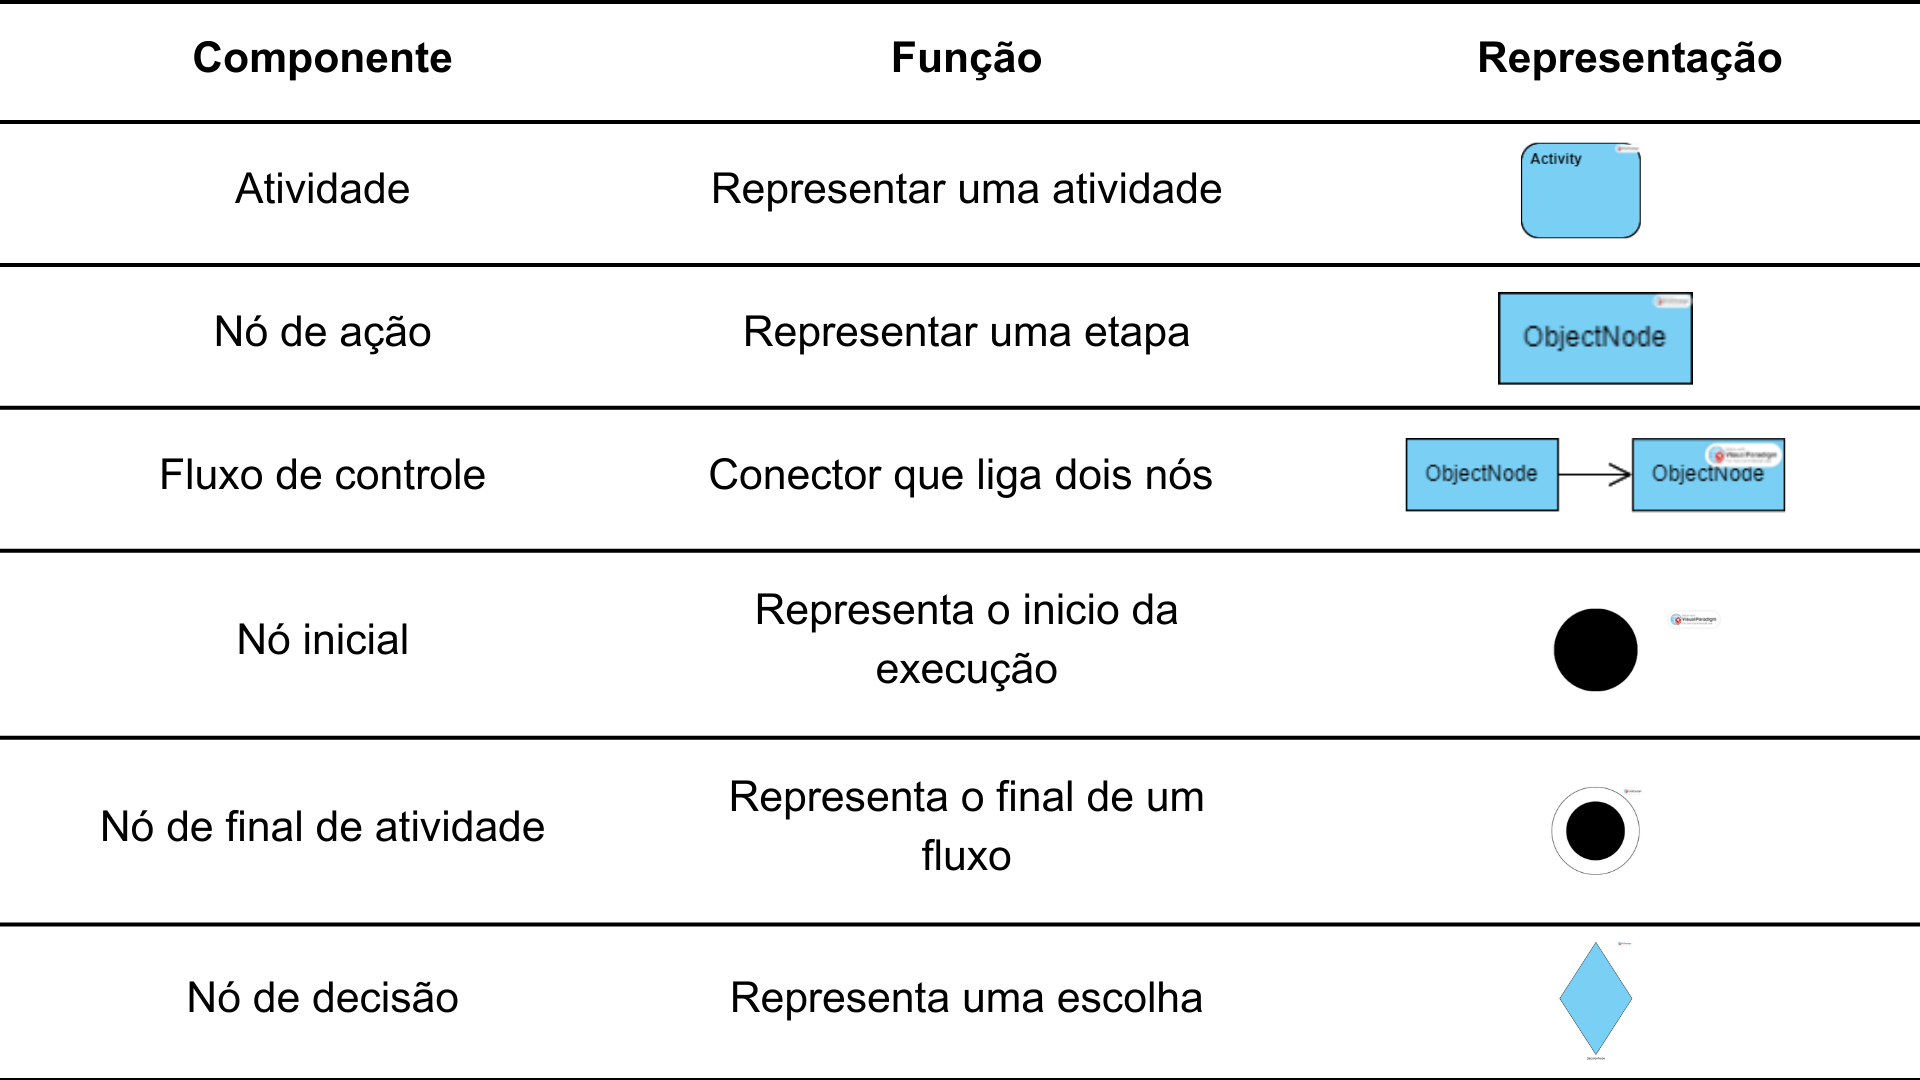
\includegraphics[scale=0.2]{img/PrincipaisCompAtividades.png}
	\\

	\footnotesize\raggedright Fonte: GUEDES(2018)
\end{figure}

\section{Exemplo do Diagrama de Atividades}

\begin{figure}[!htp]
	\caption{Exemplo de Diagrama de Atividades}
	\centering
	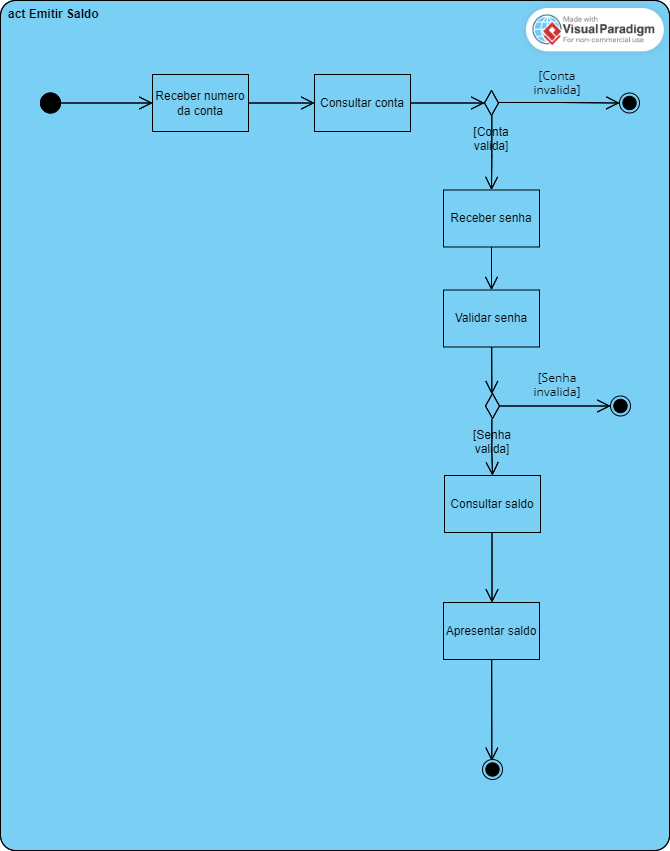
\includegraphics[scale=0.2]{img/ExemploDiagramaAtividades.png}
	\\
	\label{ExemploDiagramaAtividades}
	\footnotesize\raggedright Fonte: GUEDES(2018)
\end{figure}

Na \autoref{ExemploDiagramaAtividades} é apresentado o exemplo de emitir o saldo de uma conta: primeiramente ele recebe o número de uma determinada conta, após receber o numero da conta, chega em um nó de decisão, onde a conta é consultada, caso ela seja inválida deve-se encerrar o fluxo de atividade, caso contrário, ele passa para o nó de ação onde recebe a senha, após isso, chega a um nó de decisão onde passa a validar a senha, caso a senha seja válida, deve se encerrar o fluxo de atividade, senão deve seguir para a ação de consultar o saldo da conta, após a consulta, é apresentado na interface o saldo e a atividade é encerrada.

\chapter{Diagrama de Sequência}

\section{Objetivo do Diagrama de Sequência}

\section{Principais Componentes do Diagrama de Sequência}

\section{Exemplo do Diagrama de Sequência}

\chapter{Diagrama de Comunicação}

\section{Objetivo do Diagrama de Comunicação}

\section{Principais Componentes do Diagrama de Comunicação}

\section{Exemplo do Diagrama de Comunicação}

\chapter{Diagrama de Estrutura Composta}

\section{Objetivo do Diagrama de Estrutura Composta}

\section{Principais Componentes do Diagrama de Estrutura Composta}

\section{Exemplo do Diagrama de Estrutura Composta}

\chapter{Diagrama de Pacotes}

O diagrama de pacotes é um diagrama estrutural e tem como objetivo, segundo GUEDES(2018, pg. 274), separar as camadas de um projeto de software e descrever como os elementos estão organizados em divisões lógicas, que são chamadas de pacotes, e ainda permite modelar as subdivisões da arquitetura de uma linguagem ou de um processo de desenvolvimento.

\section{Principais Componentes do Diagrama de Pacotes}

\begin{figure}
	\caption{Representação gráfica do Pacote}
	\centering
	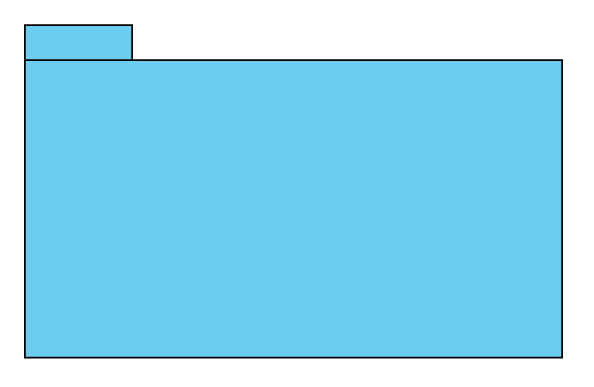
\includegraphics[scale=0.5]{img/Pacote.png}
	\\

	\label{ElementoPacote}
	\footnotesize\raggedright Fonte: Dos Autores(2024)
\end{figure}

O principal componente do diagrama de atividade é o pacote, que agrupa os elementos e nomeia esses grupos. Os pacotes podem representar sistemas, subsistemas, bibliotecas ou etapas de desenvolvimento. Um pacote pode ser contido dentro outro sem problemas. O conteúdo de um pacote não precisa ser explicitamente declarado, sendo isso desejável para poupar espaço na representação, contudo, é possível mostrar todas as informações dos conteúdos do pacote, como os métodos, atributos e relacionamentos das classes do sistema.

Um pacote pode depender de outro, existindo dois relacionamentos de dependência entre pacotes, o \textit{<<merge>>}, que indica uma combinação dos conteúdos do pacote  e o \textit{<<import>>} que indica a utilização de elementos/característica de outro pacote.  As dependências são indicadas através de setas pontilhadas, opcionalmente, com o texto \textit{<<import>>} ou \textit{<<merge>>} em cima para indicar o tipo de dependência.

Estereótipos podem ser aplicados aos pacotes para indicar o seu tipo, seja \textit{framework}, \textit{system}, \textit{subsystem} ou \textit{model}. Os estereótipos \textit{framework} e \textit{system} são representados textualmente, colocando-os antes do nome do pacote, enquanto os outros são representados graficamente.

\section{Exemplo do Diagrama de Pacotes}

\begin{figure}[!htp]
	\caption{Exemplo do Diagrama de Pacotes}
	\centering
	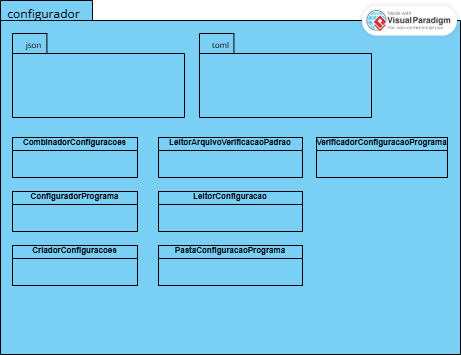
\includegraphics[scale=0.5]{img/ExemploDiagramaPacotes.png}
	\\

	\label{ExemploPacotes}
	\footnotesize\raggedright Fonte: Dos Autores(2024)
\end{figure}

A \autoref{ExemploPacotes} mostra o pacote configurador do programa heber-modelo. O diagrama mostra todos os componentes do pacote, porém não os detalha, em outras palavras, não mostra os métodos e atributos da classe, nem as relações entre elas, e não mostra os conteúdos dos subpacotes.


\chapter{Objetivos dos demais Diagramas da UML}

\section{Diagrama de Componentes}

O diagrama de componentes, de acordo com GUEDES(2018, pg. 475) é o responsável por identificar os componentes de um sistema de informação, ou de um subsistema ou os componentes e classes internas de um componente específico.

Um componente pode ser lógica(componente de negócio ou de processo) ou física(arquivos de código-fonte, arquivos de ajuda, bibliotecas, etc.).

Os diagramas de componentes são utilizados para documentar a estrutura de arquivos, facilitando a compreensão do sistema e a reutilização de código. Em especial, o diagrama de componentes é útil para gerir arquivos de configuração e mudanças nos demais arquivos do sistema.

\section{Diagrama de Implantação}

Como disse GUEDES(2018, pg. 495) o diagrama de implantação tem como enfoque a organização da arquitetura física(\textit{hardware}) sobre a qual o \textit{software} será implantado e utilizado. Ele permite demonstrar como será a distribuição dos módulos e as situações nas quais eles são executados em mais de um servidor.

Os diagramas de implantação só são úteis quando múltiplas máquinas executam os módulos ou armazenam arquivos do sistema ao mesmo tempo, caso contrário, ou seja, se o sistema rodar em apenas uma máquina não é necessário criar o diagrama de implantação.

\section{Diagrama de Tempo}

Conforme GUEDES(2018, pg. 515), o Diagrama de Tempo é similar ao Diagrama de Máquina de Estados, tendo um foco no estado de um objeto ao longo do tempo. Este diagrama é normalmente utilizado em aplicações onde o tempo é de suma importância ou que precisam de sincronia entre eventos, demonstrando os estados daquele objeto ao longo de um determinado período de tempo.

\chapter{Conclusão}

\citeoption{opcoes}
\postextual
\bibliography{referencias}

\nocite{GUEDES}
\nocite{BEZERRA}
\nocite{LARMAN}

\end{document}
